%\documentclass[class=report , crop=false, multi={itemize, figure}, float=false]{standalone}%Experimental
\documentclass[class=book , crop=false]{standalone}

\usepackage{import} % Required for importing other .tex docs.  (import uses everything bw Begin and End Doc)
\usepackage{float} % Required for specifying the exact location of a figure or table
\usepackage{graphicx} % Required for including images
\usepackage{wrapfig}
\usepackage[pdftex,breaklinks,colorlinks=true,linkcolor=black,citecolor=blue,urlcolor=red,linktocpage=false,pagebackref=true,filecolor=magenta]{hyperref}%http://www.tug.org/applications/hyperref/manual.html#x1-100003.6
\usepackage{cite}
\usepackage[toc,title,page]{appendix}
\usepackage{pdfpages} % enables loading a pdf into the doc
\usepackage{makeidx}
\usepackage{glossaries} % must be after hyperref
\usepackage{blindtext}
\usepackage{enumitem}
%\usepackage{caption}

%\setlist[description]{leftmargin=\parindent,labelindent=\parindent}

%\renewcommand*{\bibname}{References} % renames the bibliography

\newcommand{\HRule}{\rule{\linewidth}{0.5mm}} % Command to make the lines in the title page

\graphicspath{{img/}{GIS_ChampionSection/img/}{awardsChapter/GIS_ChampionSection/img/}{brandPart/awardsChapter/GIS_ChampionSection/img/}{img/}{pairedProgSection/img/}{methodChapter/pairedProgSection/img/}{methodPart/methodChapter/pairedProgSection/img/}{documentationSection/img/}{methodChapter/documentationSection/img/}{methodPart/methodChapter/documentationSection/img/}{docStorageOrgSection/img/}{methodChapter/docStorageOrgSection/img/}{methodPart/methodChapter/docStorageOrgSection/img/}{QGisSection/img/}{toolsChapter/QGisSection/img/}{servicePart/toolsChapter/QGisSection/img/}{ESRISection/img/}{toolChapter/ESRISection/img/}{servicePart/toolChapter/ESRISection/img/}{../../../../source/}{../../source/}{servicePart/applicationsChapter/treasurerSection/img/}}

%\setlength\parindent{0pt} % eliminates indents


\def\titlename{GIS Champion Award\\ \medskip\large the Code}

\title{\HRule % Horizontal Line added
\\[.4cm] % space
\begin{figure}[H] % included image
\begin{center}	% centered horizontally
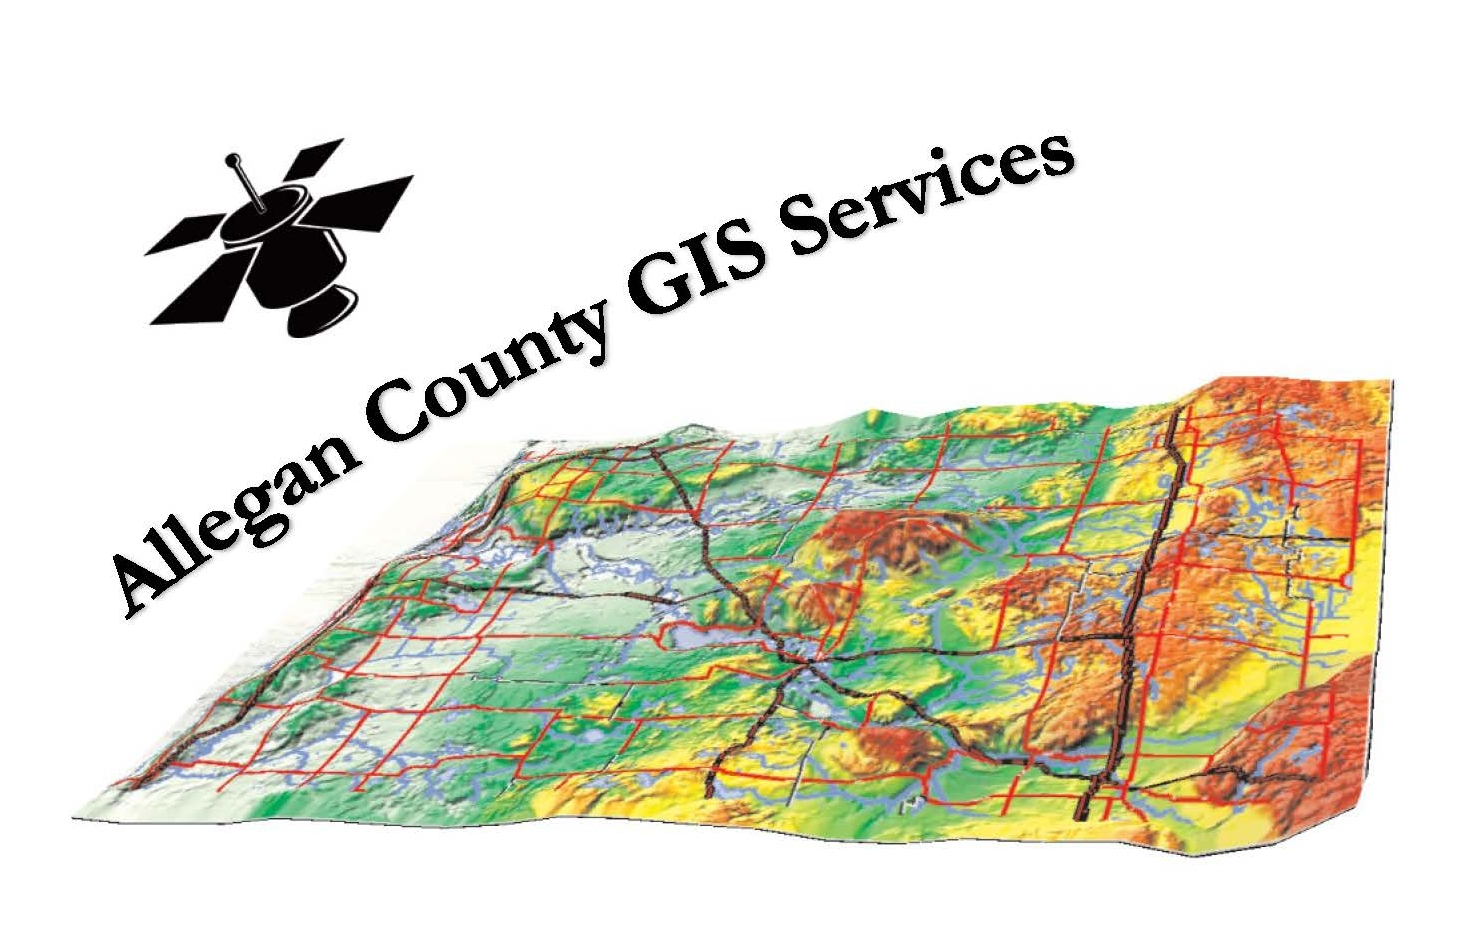
\includegraphics[scale=.45]{GIS_Logo_better.jpg}
\end{center}
\end{figure}
\Huge \bfseries \titlename \\ % Title text
\HRule \\[.4cm] % Horizontal Line added
\author{\Large Allegan County GIS \\\Large www.allegancounty.org/gis} % defines author
}  % closing brace for title

\begin{document}% Document Begins

\ifstandalone
%\frontmatter % turns off chapter numbering and uses roman numerals for page numbers
\maketitle % creates title page and blank page after title page
\tableofcontents % creates TOC and blank page
\clearpage
%\mainmatter % turns on chapter numbering, resets page numbering and uses arabic numerals for page numbers
\fi

\subsubsection{GIS Champion}
\begin{multicols}{2}
%
\paragraph{Background}
%
\noindent Treasurer department has an annual responsibility to properly document the tax forfeiture process.  \blindtext
%
\paragraph{Statement of Problem}
\noindent The current Tax Forfeiture workflow is built on MapInfo software and MS Access amd executed on a laptop pc.  \blindtext
%
\paragraph{Analysis}
\noindent \blindtext

\end{multicols}

\clearpage

\restoregeometry % reverts geometry back to original
%
\setlength{\headwidth}{\textwidth} % Set header width
\setlength{\footwidth}{\textwidth} % Set footer width
%
\paragraph{GIS Champion Award Code}
\vspace{.2in}

\begin{verbatim}
\documentclass[landscape]{article}
\usepackage{wallpaper}
\usepackage{niceframe}
\usepackage{xcolor}
\usepackage{ulem}
\usepackage{graphicx}
\usepackage{geometry}
%\geometry{tmargin=.75cm,bmargin=.25cm,
%lmargin=.8cm,rmargin=.2cm}
\geometry{tmargin=.25in,bmargin=.25in,
  lmargin=.25in,rmargin=.25in}
\usepackage{multicol}
\setlength{\columnseprule}{0.4pt}
\columnwidth=0.3\textwidth

\begin{document}
\centering
\scalebox{2.9}{
\color{green!30!black!60}
\begin{minipage}{.33\textwidth}
\font\border=umrandb
\generalframe
{\border \char113} % up left
{\border \char109} % up
{\border \char112} % up right
{\border \char108} % left
{\border \char110} % right
{\border \char114} % lower left
{\border \char111} % bottom
{\border \char115} % lower right
{\centering
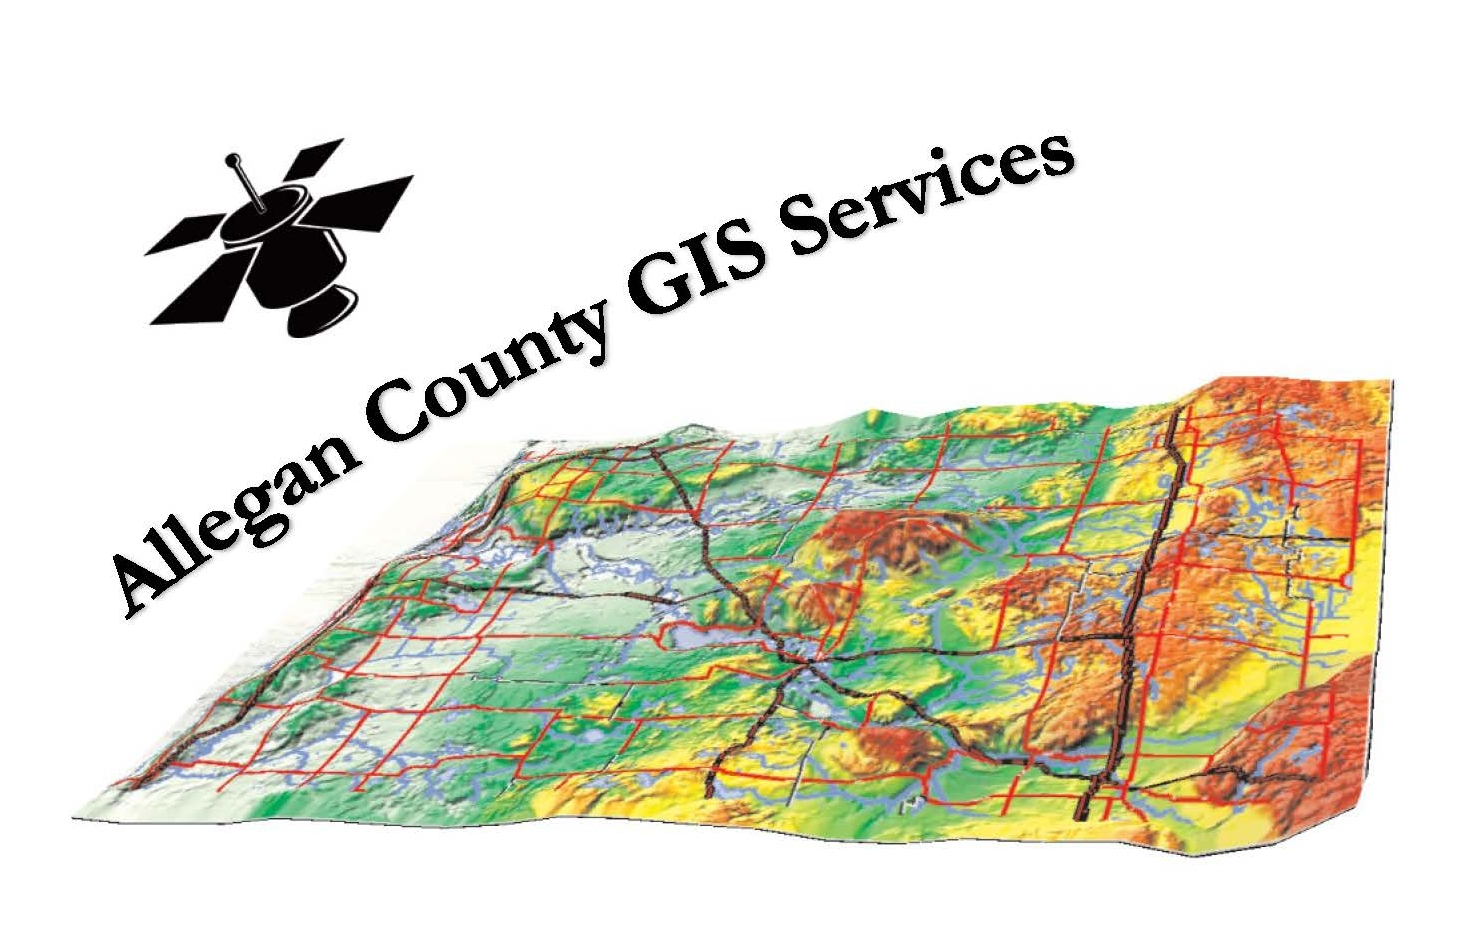
\includegraphics[height=1.5cm]{GIS_Logo_better.jpg}

\vspace{-8mm}

\curlyframe[.9\columnwidth]{

\textcolor{green!10!black!90}
{\small Allegan County GIS Services}
\vspace{.005in}

\textcolor{green!10!black!90}{
\tiny Recognizes}\\
%\smallskip
\vspace{.005in}
\uline{\textcolor{green!30!black!60}
\textcolor{green!30!black!60}{Brian Redmond}}
\\
\smallskip
\tiny Information Services Technician

%\smallskip
\textcolor{green!10!black!90}
{
\\
\tiny for Excellence in
}
\smallskip
\\
\textcolor{black}{\normalsize \textsc{Enabling
 Employee Experiences}}
\\
\vspace{.1in}
\textcolor{green!10!black!90}
{
\tiny on this day
\itshape September 21, 2018
}

\vspace{.1in}

{\color{green!10!black!90}
\scalebox{.6}{

\begin{tabular}{ccc}
\cline{1-1}
\cline{3-3}
\\
Neil Besteman  & &  Bryan May \\
GIS Manager & & GIS Analyst \\
\end{tabular}

} % closes scalebox{.6} arg
} % closes blue!40!black
} % closes curlyframe arg
} % closes centering
\end{minipage}
} % closes scalebox{2.8} arg

\end{document}
\end{verbatim}

\end{document}
